% =============================== 4. Q1 ===============================
\section{Question 1: A Behavioural Model of Riding}\label{sec:q1}

The deliverable of Q1 is a probability law for a trip: when it starts, where it goes,
and how long it lasts. We build it in three layers --- generation, destination,
duration --- and validate the layers jointly against held-out days.

\subsection{Generation: a non-homogeneous Poisson process}

Each cell $i$ emits trips as a Poisson process whose rate $\lambda_{i}(t)$ is constant
on 15-minute intervals. The rate is estimated by the sample mean of the counts in that
interval over the seven typical days,
\begin{equation}
\hat\lambda_{it} \;=\; \frac{1}{7}\sum_{k=1}^{7} N_{it}^{(k)},
\end{equation}
where $N^{(k)}_{it}$ is the number of departures from cell $i$ in interval $t$ on day
$k$. With 5,263 cells and 96 intervals the table has $5.05\times10^{5}$ entries, which
is precisely the level of detail the data support: the average cell-interval contains
0.54 trips, and the profile (\figref{fig:data}b) is bimodal on weekdays, with a sharp
8 a.m. peak, a lunchtime shoulder and an evening peak at 6 p.m., and unimodal on
weekends.

\subsection{Destination: a singly-constrained gravity model}

Conditional on departing from $i$ in time band $h$, a rider chooses destination $j$
with probability
\begin{equation}
P(j\mid i,h) \;=\; \frac{A_j(h)\,e^{-\beta_h d_{ij}}}
                        {\sum_{k} A_k(h)\,e^{-\beta_h d_{ik}}},
\qquad d_{ij}\ \text{in km},
\label{eq:gravity}
\end{equation}
where $A_j(h)$ is the attraction of $j$ in band $h$ and $\beta_h>0$ is the distance
decay. The model is origin-constrained --- the probabilities sum to one over
destinations for every origin --- so the observed origin totals are reproduced exactly
and no balancing procedure is required beyond the denominator.

The exponential form is not an arbitrary choice. If trips are the most probable
allocation of $n_{ih}=\sum_j n_{ijh}$ indistinguishable riders to destinations subject
to a known mean trip length, the maximum-entropy distribution is
\cite{wilson1970}
\begin{equation}
n_{ijh} \;\propto\; A_j(h)\,e^{-\beta_h d_{ij}},
\end{equation}
and $\beta_h$ is the Lagrange multiplier of the distance constraint. It measures how
strongly riders resist distance: a large $\beta_h$ means the destination distribution
is concentrated near the origin.

Attraction is measured, not assumed. We set
\begin{equation}
A_j(h) \;=\; \sum_{n:\,h_n=h} K\!\left(\|c_j-c_{d_n}\|\right),
\end{equation}
a Gaussian kernel ($\sigma=1.2$ cells, about 600 m) over the destinations actually
observed in band $h$, evaluated at the cell centroid $c_j$. The kernel matters because
a destination's pull extends beyond its own cell boundary: a rider heading for a
shopping street will accept any of the cells that front it. Using unsmoothed arrival
counts instead would set $A_j=0$ for 0.3\% of cells in the busiest bands and for 30.6\%
of them at night, forbidding trips that the data plainly contain.

\subsection{Estimation}

Only $\beta_h$ is a free parameter. For a band with trips $\{(i_n,j_n)\}$ it is the
maximiser of the conditional log-likelihood
\begin{equation}
\ell(\beta) \;=\; \sum_{n} \left[\log A_{j_n}(h) - \beta\, d_{i_n j_n}
 - \log \sum_k A_k(h)\,e^{-\beta d_{i_n k}}\right],
\label{eq:mle}
\end{equation}
which is concave in $\beta$; we maximise it by bounded scalar search
\cite{virtanen2020}. The five bands are estimated separately on five randomly chosen
typical days and tested on the remaining two. \tabref{tab:q1} reports the estimates and
the out-of-sample performance.

\begin{table}[htbp]
\centering
\caption[Q1 estimates and held-out performance]{Q1 estimates and out-of-sample performance (two held-out days). Log-loss is
nats per trip; lower is better. ``Attraction only'' is the same model with
$\beta_h=0$.}
\label{tab:q1}
\small
\begin{tabular}{@{}lrrrrrrr@{}}
\toprule
\textbf{Band} & \textbf{Train trips} & $\hat\beta_h$ & \textbf{Gravity} &
\textbf{Distance} & \textbf{Attraction} & \textbf{Uniform} & \textbf{Top-5 hit} \\
 & & (km$^{-1}$) & \textbf{log-loss} & \textbf{only} & \textbf{only} & & \textbf{gravity / dist.} \\
\midrule
00--05 & 18,364 & 2.096 & 3.313 & 3.488 & 7.912 & 8.568 & 0.476 / 0.401 \\
06--09 & 386,102 & 2.014 & 3.512 & 3.646 & 8.083 & 8.568 & 0.399 / 0.339 \\
10--15 & 366,212 & 2.517 & 3.239 & 3.279 & 8.091 & 8.568 & 0.458 / 0.441 \\
16--19 & 428,478 & 2.130 & 3.517 & 3.562 & 8.140 & 8.568 & 0.408 / 0.383 \\
20--23 & 165,671 & 2.364 & 3.360 & 3.395 & 8.185 & 8.568 & 0.455 / 0.438 \\
\bottomrule
\end{tabular}
\end{table}

Three readings of \tabref{tab:q1} matter.

\textbf{Distance is the dominant explanatory variable.} The attraction-only model is
almost useless --- its log-loss is close to the uniform benchmark over 5,263
destinations ($\log 5263=8.57$) --- because in a balanced system the marginal number of
arrivals at a cell says little about where any particular rider is going. Distance
alone already reaches a log-loss of 3.28--3.65.

\textbf{Attraction adds a consistent but modest gain.} Adding $A_j(h)$ improves the
log-loss by 0.035--0.175 nats and the top-five hit rate by 1.7--7.5 percentage points
in every band and on held-out days. The gain is largest in the small hours, when the
destination choice is least constrained by commuting routine, and smallest in the late
evening, when the distance term is already sharp.

\textbf{The decay varies by time of day, and in the expected direction.} Morning has
the weakest decay ($\hat\beta=2.01$): the morning trip is the commute, and commutes are
long. Midday has the strongest ($\hat\beta=2.52$): the midday trip is an errand, and
errands are local. The evening sits between, and late evening recovers some of the
morning's reach as riders return home. This is the behavioural content of the model,
and it is what makes a time-varying formulation necessary: a single $\beta$ would
average the commute and the errand and misdescribe both.

\subsection{Duration}

Ride duration is generated from speed rather than modelled directly. A bicycle travels
the street network, which is about 1.35 times the straight-line distance at the
distances observed here; the speed of a dockless rider is approximately normal with
mean 11.5 km/h and standard deviation 2.5, clipped to $[6,20]$ km/h to remove the
implausible tails. Hence
\begin{equation}
\tau_n \;=\; \frac{1.35\,d_n}{v_n}\times 60 + 1 \quad \text{minutes},
\label{eq:dur}
\end{equation}
with the additive minute standing for locking and unlocking. The resulting
distribution has median 5.9 minutes, 10th percentile 3.0 and 90th percentile 11.9,
which matches the observed distribution of within-day ride durations.

\subsection{Joint validation}

The layers are estimated separately but must be checked together: a model can fit each
margin and still produce impossible trips. We therefore simulate a full typical day
--- draw each trip's time from the Poisson rates, its destination from
\eqnref{eq:gravity}, its duration from \eqnref{eq:dur} --- and compare the simulated
trip-length distribution with the observed one (\figref{fig:q1}a). The two-sample
Kolmogorov--Smirnov statistic is 0.196, and the discrepancy is confined to the
shortest trips, exactly where the geohash floor sits. Given that the model reproduces
the distance distribution, the hourly profile (by construction) and the destination
choice (by the held-out test), it is adequate as the demand engine for Q2--Q4.

\begin{figure}[htbp]
\centering
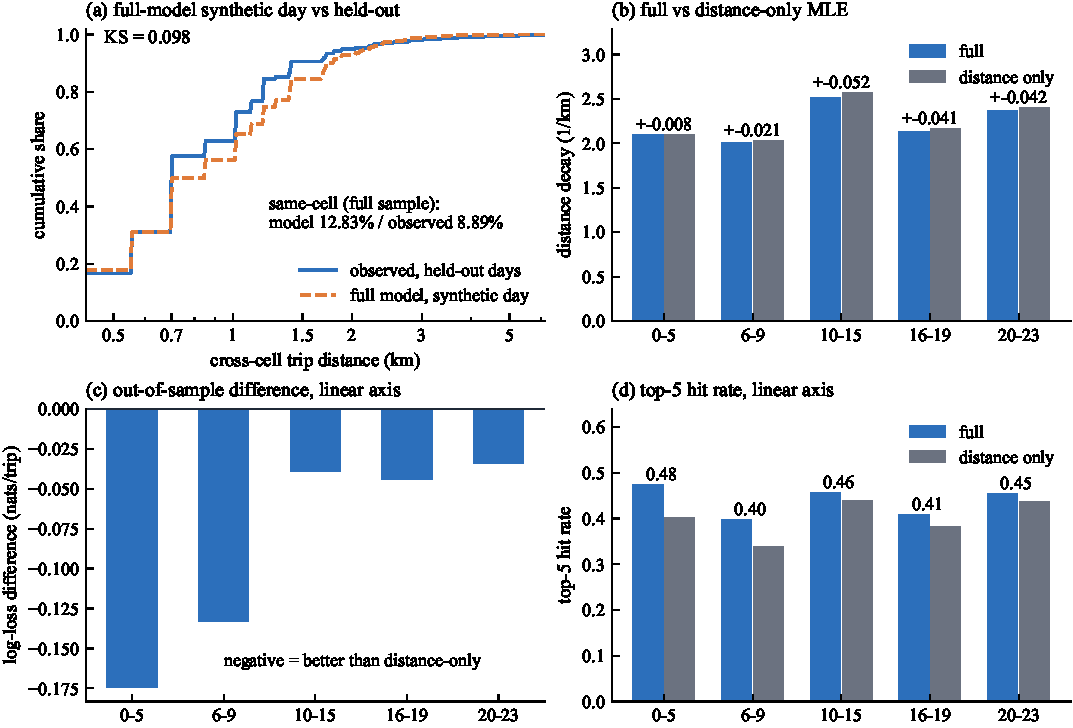
\includegraphics[width=0.9\linewidth]{../figs/fig3_q1_validation.pdf}
\caption[Q1 validation]{Q1 validation. (a) Simulated against observed trip-length distributions.
(b) Estimated distance decay by time band. (c) Out-of-sample log-loss for three
model specifications, logarithmic scale. (d) Top-five destination hit rate.}
\label{fig:q1}
\end{figure}

\subsection{Who is riding}

A single representative rider would misrepresent the system, because the hourly
profile is the superposition of distinct behaviours. We characterise each user by six
features computed over the ten usable days: trips per day, mean trip distance, entropy
of the departure-hour distribution, share of trips in peak hours, share on weekends,
and share of trips that return to the origin cell. $k$-means \cite{lloyd1982} with the
silhouette criterion \cite{rousseeuw1987} selects $k=5$ (silhouette 0.256; the
alternatives $k=3$ and $k=4$ score 0.239 and 0.237), and the resulting classes are
stable across random initialisations.

\begin{table}[htbp]
\centering
\caption[Latent user segments]{Latent user segments (ten days). ``Peak'' is the share of a user's trips
starting in 07--09 or 17--19.}
\label{tab:seg}
\small
\begin{tabular}{@{}lrrrrrr@{}}
\toprule
\textbf{Segment} & \textbf{Users} & \textbf{Share of} & \textbf{Share of} &
\textbf{Trips} & \textbf{Distance} & \textbf{Weekend} \\
 & & \textbf{users} & \textbf{trips} & \textbf{per day} & \textbf{(km)} & \textbf{share} \\
\midrule
Regular multi-purpose & 132,984 & 40.4\% & 51.8\% & 9.18 & 0.84 & 0.19 \\
Heavy short-trip & 49,931 & 15.2\% & 29.6\% & 13.98 & 0.67 & 0.20 \\
Commuter & 67,528 & 20.5\% & 10.6\% & 3.71 & 1.17 & 0.07 \\
Low frequency & 49,396 & 15.0\% & 5.2\% & 2.48 & 0.89 & 0.03 \\
Weekend / leisure & 29,410 & 8.9\% & 2.8\% & 2.25 & 0.92 & 0.79 \\
\bottomrule
\end{tabular}
\end{table}

\figref{fig:seg} and \tabref{tab:seg} show the structure. Two groups generate
four-fifths of all trips. The \emph{regular multi-purpose} user rides 9.2 times a day
--- the profile of a short-distance commuter or a rider who uses the bicycle as a
substitute for walking --- and accounts for 51.8\% of trips. The \emph{heavy
short-trip} user rides 14 times a day over 0.67 km, with a quarter of trips returning
to the same cell: this is the courier-like, errand-heavy behaviour that dominates the
dense core. The \emph{commuter} class rides longer (1.17 km) and concentrates 91\% of
its trips in peak hours but contributes only 10.6\% of volume. The remaining two
classes are peripheral.

This matters operationally rather than descriptively. The peak is made by a minority
of trips --- commuters, 10.6\% of volume --- while the volume is made by riders whose
trips are short and whose destinations are diffuse. An intervention designed to
flatten the peak must target the first group; one designed to reduce total vehicle
movement must target the second. Neither can be inferred from the aggregate profile,
which is why the segmentation is part of the deliverable.

\begin{figure}[htbp]
\centering
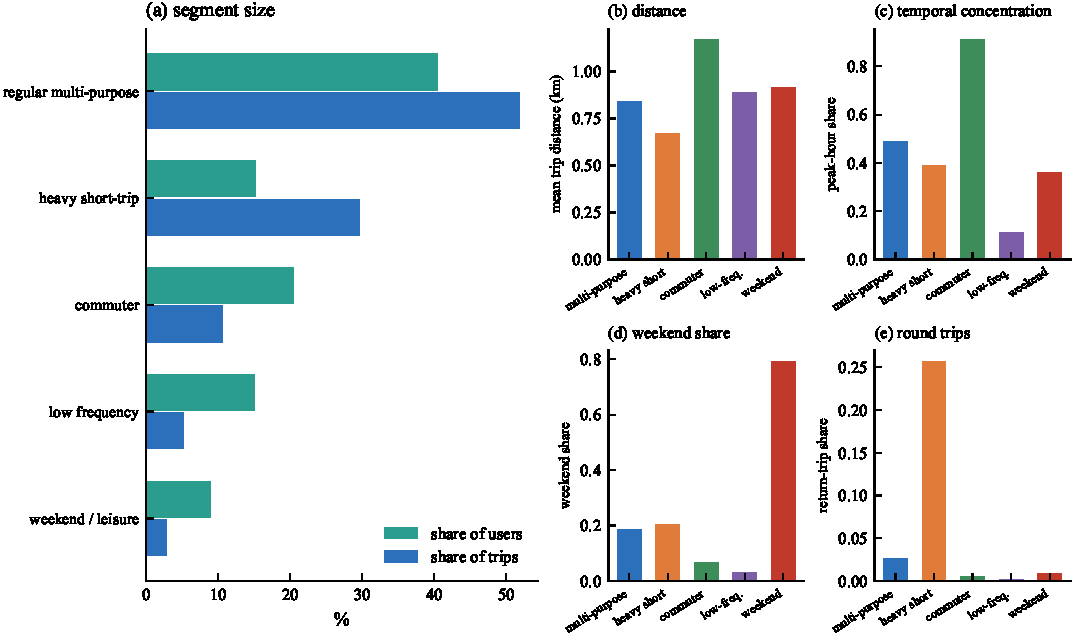
\includegraphics[width=0.9\linewidth]{../figs/fig2_segments.pdf}
\caption[User segments]{User segments. (a) Size of each segment by users and by trips. (b)--(e)
Behavioural signature on four dimensions.}
\label{fig:seg}
\end{figure}
